%%%%%%%%%%%%%%%%%%%%%%%%%%%%%%%%%%%%%%%%%%%%%%%%%%%%%%%%%%%%%%%%%%%%%%%%%%%%%%%%
%         National Institute of Electronics and Information Technology (NIELIT)
%                      Gorakhpur Centre, Uttar Pradesh
%          NIELIT Internship Project Report --- Custom LaTeX Class
%
%  Project: QR Attendance System
%  Author: Tanya Singh
%%%%%%%%%%%%%%%%%%%%%%%%%%%%%%%%%%%%%%%%%%%%%%%%%%%%%%%%%%%%%%%%%%%%%%%%%%%%%%%%

\documentclass{SOICTthesis}

% ========================
% Thesis Information Setup
% ========================
\thesistitle{QR Attendance System --- A Dynamic QR-Based Student Attendance Management System}
\degree{Internship Program}
\program{Information Technology}
\specialization{Web Application Development}
\authorname{Tanya Singh}
\enrollmentno{NIELIT/GKP/2026}
\supervisor{NIELIT Faculty}{Supervisor}
\university{NIELIT Gorakhpur Centre}
\submissiondate{March 2026}

% ================
% Packages
% ================
\RequirePackage{booktabs}
\RequirePackage{multirow}

\begin{document}

% ====================
% Abstract Section
% ====================
\theabstract{
Attendance management is a fundamental administrative activity in educational institutions. Traditional methods such as manual roll calls and paper-based registers are time-consuming, prone to errors, and susceptible to proxy attendance. This project presents a full-stack web-based attendance management system that leverages dynamic QR codes to address these challenges. The system generates QR codes that automatically rotate every 15 seconds, ensuring that only students physically present in the classroom at that moment can mark their attendance by scanning the code with their mobile phones. The application features three distinct user portals --- Student Portal (for QR scanning), Teacher/Faculty Portal (for QR generation, daily and monthly attendance views), and Admin Panel (for managing teachers, students, and courses). The backend is powered by Supabase Edge Functions (TypeScript on Deno runtime) with PostgreSQL as the database, while the frontend is built using React 18 with Vite 5. The system includes JWT-based authentication, role-based access control, real-time attendance tracking with exact scan timestamps, calendar-style monthly PDF reports using jsPDF, and CSV export capabilities. The application is deployed on Netlify (frontend) and Supabase Cloud (backend), ensuring 24/7 accessibility. Key outcomes include elimination of proxy attendance, automated report generation, and a scalable multi-course architecture.
}

% ====================
% Chapters Begin Here
% ====================

% ---------------------------------
\chapter{INTRODUCTION}
\label{ch:introduction}
% ---------------------------------

\section{Background}
\label{sec:background}

Attendance management is a fundamental administrative activity in educational institutions worldwide. Maintaining accurate attendance records is essential for monitoring student engagement, ensuring academic compliance, and generating official reports. Traditional methods of attendance tracking, such as manual roll calls and paper-based registers, have been used for decades but suffer from several significant limitations.

Manual roll calls consume valuable lecture time, often taking 5-10 minutes at the start of each session. Paper registers can be easily manipulated, enabling proxy attendance where one student marks attendance on behalf of an absent peer. Additionally, paper-based systems offer no audit trail to verify when attendance was actually marked, and generating monthly or semester-level reports from paper registers requires tedious manual compilation that is both time-consuming and error-prone.

With the rapid advancement of web technologies, mobile devices, and cloud computing, there is a strong need for a digital, secure, and efficient attendance tracking solution that can operate across devices and provide real-time data access. QR (Quick Response) code technology, combined with modern web application frameworks, presents an ideal solution to these challenges.

The National Institute of Electronics and Information Technology (NIELIT) conducts various courses simultaneously with different teachers and student batches. An institution of this scale requires a robust attendance management system that supports multiple courses, provides role-based access for different user types, and generates automated reports for administrative purposes.

\section{Problem Statement}
\label{sec:problem_statement}

The existing attendance management practices at educational institutions face the following critical challenges:

\begin{itemize}
    \item \textbf{Time consumption:} Manual roll calls consume valuable lecture time, reducing effective teaching hours.
    \item \textbf{Proxy attendance:} Paper-based systems are easily manipulated, with students marking attendance for absent peers.
    \item \textbf{No audit trail:} There is no mechanism to verify the exact time when attendance was recorded.
    \item \textbf{Manual report generation:} Consolidating daily attendance into monthly or semester reports is tedious and error-prone.
    \item \textbf{Multi-course complexity:} Institutions running multiple courses with different teachers need a centralised yet course-specific attendance solution.
    \item \textbf{No real-time visibility:} Teachers and administrators lack real-time access to attendance statistics and trends.
\end{itemize}

\section{Objectives of the Assigned Work}
\label{sec:objectives}

The specific objectives of this internship project are:

\begin{enumerate}
    \item To develop a secure, web-based attendance management system using dynamic QR codes that rotate every 15 seconds to prevent proxy attendance.
    \item To create separate portals for Students, Teachers, and Administrators with role-based access control.
    \item To enable real-time attendance tracking with exact scan timestamps for audit purposes.
    \item To provide comprehensive daily and monthly attendance reporting capabilities.
    \item To implement PDF and CSV export functionality for official record-keeping.
    \item To ensure the system works across devices including mobile phones for QR scanning.
    \item To deploy the application on cloud infrastructure for 24/7 accessibility.
    \item To design a scalable database schema supporting multiple courses and teachers.
\end{enumerate}

\section{Scope of the Project}
\label{sec:scope}

This project encompasses the complete design, development, testing, and deployment of a QR-based attendance management system. The scope includes:

\begin{itemize}
    \item A React-based Single Page Application (SPA) with responsive design.
    \item Three Supabase Edge Functions for backend API operations.
    \item A PostgreSQL database with four primary tables and eight migration files.
    \item JWT-based authentication with Supabase Auth.
    \item Dynamic QR code generation and camera-based scanning.
    \item Monthly attendance report with PDF export (calendar-style grid with NIELIT branding).
    \item CSV export for data portability.
    \item Deployment on Netlify (frontend) and Supabase Cloud (backend).
\end{itemize}

\section{Organization of the Report}
\label{sec:organization}

The remainder of this report is organised as follows: Chapter~2 details the work allocated and completed during the internship. Chapter~3 describes the technology stack and tools used. Chapter~4 explains the methodology adopted including system architecture, database design, and development approach. Chapter~5 presents the implementation details. Chapter~6 discusses the outcomes and key learnings from the project. Chapter~7 provides the conclusion and future scope.


% ---------------------------------
\chapter{DETAILS OF WORK ALLOCATED AND COMPLETED}
\label{ch:work_details}
% ---------------------------------

\section{Work Allocated}
\label{sec:work_allocated}

The following work was allocated as part of the NIELIT internship program:

\begin{enumerate}
    \item Design and develop a complete web-based student attendance system.
    \item Implement QR code-based attendance marking with anti-proxy mechanisms.
    \item Create a multi-role application with Admin, Teacher, and Student interfaces.
    \item Develop backend API services for attendance management operations.
    \item Design and implement a PostgreSQL database schema for the system.
    \item Build PDF and CSV export functionality for attendance reports.
    \item Deploy the application on cloud infrastructure for production use.
    \item Write documentation and prepare a project presentation.
\end{enumerate}

\section{Work Completed}
\label{sec:work_completed}

All allocated work was successfully completed. Table~\ref{tab:work_completed} provides a summary of each module and its completion status.

\begin{table}[H]
\centering
\caption{Summary of Work Completed}
\label{tab:work_completed}
\begin{tabular}{|c|p{3cm}|p{7.5cm}|c|}
    \hline
    \textbf{S.No} & \textbf{Module} & \textbf{Description} & \textbf{Status} \\
    \hline
    1 & User Authentication & Login, registration, password reset with Supabase Auth + JWT & Done \\
    \hline
    2 & Student Portal & QR camera scanning, attendance confirmation, personal history & Done \\
    \hline
    3 & Teacher Portal & QR generation, daily/monthly views, attendance session management & Done \\
    \hline
    4 & Admin Panel & CRUD for teachers, students, courses; dashboard statistics & Done \\
    \hline
    5 & Backend API & 3 Supabase Edge Functions: attendance-api, manage-users, mark-attendance & Done \\
    \hline
    6 & Database Design & PostgreSQL tables: students, courses, attendance, profiles + 8 migrations & Done \\
    \hline
    7 & PDF/CSV Export & Calendar-style monthly PDF with NIELIT branding + CSV export & Done \\
    \hline
    8 & Deployment & Netlify (frontend CI/CD) + Supabase Cloud (backend + database) & Done \\
    \hline
\end{tabular}
\end{table}


% ---------------------------------
\chapter{TECHNOLOGY STACK AND TOOLS}
\label{ch:tech_stack}
% ---------------------------------

\section{Frontend Technologies}
\label{sec:frontend_tech}

\begin{table}[H]
\centering
\caption{Frontend Technologies Used}
\label{tab:frontend_tech}
\begin{tabular}{|l|c|p{7cm}|}
    \hline
    \textbf{Technology} & \textbf{Version} & \textbf{Purpose} \\
    \hline
    React.js & 18.2 & Core UI library for building interactive SPA \\
    \hline
    Vite & 5.0 & Fast build tool and dev server with HMR \\
    \hline
    React Router & 6.20 & Client-side routing between portals \\
    \hline
    html5-qrcode & 2.3.8 & Camera-based QR code scanning \\
    \hline
    qrcode & 1.5.3 & QR code generation for teachers \\
    \hline
    jsPDF & 2.5.1 & Client-side PDF generation for reports \\
    \hline
    Supabase JS & 2.39 & Client SDK for Supabase Auth and API \\
    \hline
\end{tabular}
\end{table}

\section{Backend Technologies}
\label{sec:backend_tech}

\begin{table}[H]
\centering
\caption{Backend Technologies Used}
\label{tab:backend_tech}
\begin{tabular}{|p{4.5cm}|p{8cm}|}
    \hline
    \textbf{Technology} & \textbf{Purpose} \\
    \hline
    Supabase Edge Functions (Deno/TypeScript) & Serverless API endpoints for all backend operations \\
    \hline
    Supabase Auth & User authentication with JWT tokens, email-based login \\
    \hline
    PostgreSQL & Relational database for students, attendance, courses, profiles \\
    \hline
    Row Level Security (RLS) & Database-level access control policies \\
    \hline
\end{tabular}
\end{table}

\section{DevOps and Deployment Tools}
\label{sec:devops}

\begin{itemize}
    \item \textbf{Netlify:} Frontend hosting with automatic CI/CD from GitHub pushes.
    \item \textbf{Supabase Cloud:} Managed PostgreSQL database, Auth, and Edge Functions hosting.
    \item \textbf{Git and GitHub:} Version control and source code repository management.
    \item \textbf{VS Code:} Primary development IDE with extensions for React, TypeScript, and Git.
    \item \textbf{Chrome DevTools:} Frontend debugging, network inspection, and performance analysis.
\end{itemize}


% ---------------------------------
\chapter{METHODOLOGY ADOPTED}
\label{ch:methodology}
% ---------------------------------

\section{Development Approach}
\label{sec:dev_approach}

The project followed an \textbf{Agile development methodology} with iterative development cycles. Given the internship timeframe, the work was organised into focused sprints, each delivering a functional increment of the system.

\subsection{Phase 1: Requirements Analysis and Design}
Understanding the attendance management requirements at NIELIT, identifying use cases for each user role (Admin, Teacher, Student), designing the database schema, and planning the system architecture. The three-tier architecture (Presentation, Application, Data) was selected for modularity and scalability.

\subsection{Phase 2: Backend Development}
Setting up the Supabase project, creating PostgreSQL tables, writing Edge Functions for authentication, attendance management (mark-attendance, mark-self, get-daily, get-monthly, finalize), and user management (CRUD operations for teachers, students, and courses).

\subsection{Phase 3: Frontend Development}
Building the React SPA with Vite, developing individual components (Login, StudentPortal, TeacherPortal, AdminPanel, QRScanner, Navigation), integrating QR code generation and scanning libraries, and implementing responsive UI design.

\subsection{Phase 4: Integration and Testing}
Connecting frontend to backend APIs, testing QR scanning across devices (laptop camera, mobile phone), validating time-window logic, testing edge cases (duplicate marking, expired QR, wrong course), and fixing bugs.

\subsection{Phase 5: Report Generation Module}
Implementing the monthly attendance report with calendar-style PDF export using jsPDF, adding CSV export, building the interactive monthly dashboard with daily attendance grid showing Present/Absent/Weekend status for each day.

\subsection{Phase 6: Deployment and Documentation}
Deploying the frontend on Netlify with CI/CD from GitHub, configuring Supabase Edge Functions for production, writing project documentation, and preparing the internship report and presentation.

\section{System Architecture}
\label{sec:system_architecture}

The QR Attendance System follows a \textbf{three-tier architecture} consisting of a Presentation Layer (frontend), Application Layer (backend API), and Data Layer (database).

\begin{itemize}
    \item \textbf{Presentation Layer:} React 18 + Vite 5 SPA deployed on Netlify. Contains Student Portal (QR scanning), Teacher Portal (QR generation, reports), and Admin Panel (CRUD, dashboard).
    \item \textbf{Application Layer:} Supabase Edge Functions (Deno/TypeScript), serverless. Three functions: \texttt{attendance-api} (mark, get-daily, get-monthly, finalize), \texttt{manage-users} (CRUD), \texttt{mark-attendance} (QR RPC).
    \item \textbf{Data Layer:} PostgreSQL (Supabase) with Supabase Auth (JWT). Tables: students, courses, attendance, profiles. Row Level Security for data isolation.
\end{itemize}

\section{Database Design}
\label{sec:database_design}

The system uses PostgreSQL with four primary tables:

\subsection{Students Table}

\begin{table}[H]
\centering
\caption{Students Table Schema}
\label{tab:students_schema}
\begin{tabular}{|l|l|p{6cm}|}
    \hline
    \textbf{Column} & \textbf{Type} & \textbf{Description} \\
    \hline
    id & SERIAL (PK) & Auto-incrementing primary key \\
    \hline
    roll\_number & VARCHAR & Unique roll number per course \\
    \hline
    name & VARCHAR & Student full name \\
    \hline
    email & VARCHAR & Student email address \\
    \hline
    course\_code & VARCHAR & Course code reference (e.g., JAI-001) \\
    \hline
    user\_id & UUID & Reference to Supabase Auth user \\
    \hline
\end{tabular}
\end{table}

\subsection{Attendance Table}

\begin{table}[H]
\centering
\caption{Attendance Table Schema}
\label{tab:attendance_schema}
\begin{tabular}{|l|l|p{6cm}|}
    \hline
    \textbf{Column} & \textbf{Type} & \textbf{Description} \\
    \hline
    id & VARCHAR (PK) & Composite key: \{student\_id\}-\{date\} \\
    \hline
    student\_id & INTEGER (FK) & References students.id \\
    \hline
    date & DATE & Attendance date (YYYY-MM-DD) \\
    \hline
    status & VARCHAR & `present'' or `absent'' \\
    \hline
    scan\_time & TIMESTAMP & Exact ISO timestamp of QR scan \\
    \hline
    finalized & BOOLEAN & Whether attendance is locked \\
    \hline
\end{tabular}
\end{table}

\subsection{Courses Table}
Stores course information with teacher assignment. Fields: \textbf{course\_code} (PK), \textbf{course\_name}, \textbf{teacher\_id} (UUID), \textbf{teacher\_name}.

\subsection{Profiles Table}
Stores user roles mapped to Supabase Auth UUIDs. Fields: \textbf{id} (UUID, PK), \textbf{role} (admin / teacher / student). This table enables role-based access control.

\subsection{Database Migrations}
The project includes 8 database migration files applied sequentially to evolve the schema:

\begin{enumerate}
    \item Add email column to students table.
    \item Fix students user\_id type to UUID.
    \item Add unique constraint on students user\_id.
    \item Fix roll\_number uniqueness constraint per course.
    \item Allow students to enroll in multiple courses.
    \item Cleanup orphan student records.
    \item Ensure correct constraints on all tables.
    \item Complete reset and rebuild of students table schema.
\end{enumerate}


% ---------------------------------
\chapter{IMPLEMENTATION DETAILS}
\label{ch:implementation}
% ---------------------------------

\section{QR Code Attendance Flow}
\label{sec:qr_flow}

The core innovation of this system is the dynamic QR code-based attendance mechanism. The flow works as follows:

\begin{enumerate}
    \item \textbf{Start Session:} Teacher logs into the Faculty Portal and clicks `Start Attendance Session''.
    \item \textbf{QR Generation:} The system generates a QR code containing: \texttt{ATTENDANCE|teacher\_id|timestamp\_ms}.
    \item \textbf{Auto-Rotation:} The QR code automatically regenerates every 15 seconds with a fresh timestamp.
    \item \textbf{Student Scan:} Students open the Student Portal on their mobile phones and scan the QR code using their camera.
    \item \textbf{Backend Validation:} The backend validates: (a) QR format correctness, (b) timestamp within 30 seconds, (c) teacher teaches the student's course, (d) student hasn't been marked today.
    \item \textbf{Record Creation:} On successful validation, an attendance record is inserted with status=`present'' and the exact scan timestamp.
    \item \textbf{Real-Time Update:} The teacher's dashboard updates in real-time showing Present/Absent/Total counts.
\end{enumerate}

\section{Frontend Components}
\label{sec:frontend_components}

The frontend is organised into the following React components:

\begin{itemize}
    \item \textbf{Login.jsx:} Authentication page with email/password login and role-based redirection.
    \item \textbf{StudentPortal.jsx:} Student interface for QR scanning and viewing personal attendance.
    \item \textbf{TeacherPortal.jsx:} Faculty interface with tabs --- Show QR Code, Daily View, Monthly Report.
    \item \textbf{AdminPanel.jsx:} Administrative dashboard for managing teachers, students, and courses.
    \item \textbf{QRScanner.jsx:} Reusable QR code camera scanning component using html5-qrcode.
    \item \textbf{Navigation.jsx:} Top navigation bar with user info, role badge, and logout.
    \item \textbf{ForgotPassword.jsx:} Password recovery via email.
    \item \textbf{ResetPassword.jsx:} Token-based password reset form.
    \item \textbf{ChangePassword.jsx:} In-app password change for authenticated users.
\end{itemize}

\section{Backend Edge Functions}
\label{sec:edge_functions}

\begin{table}[H]
\centering
\caption{Supabase Edge Functions}
\label{tab:edge_functions}
\begin{tabular}{|p{3cm}|p{5cm}|p{4.5cm}|}
    \hline
    \textbf{Function} & \textbf{Actions} & \textbf{Description} \\
    \hline
    attendance-api & server-time, mark-attendance, mark-self, get-daily, get-monthly, get-courses, finalize & Core attendance operations \\
    \hline
    manage-users & list, delete, create (teacher/student) & User and course CRUD for admin \\
    \hline
    mark-attendance & QR RPC call & Direct QR-based marking via RPC \\
    \hline
\end{tabular}
\end{table}

\section{PDF Report Generation}
\label{sec:pdf_generation}

The monthly attendance PDF is generated client-side using jsPDF in landscape orientation. Features include:

\begin{itemize}
    \item NIELIT institutional header with organization name.
    \item Course code, course name, faculty name, month/year metadata.
    \item Calendar-style grid with columns for days 1--31.
    \item Per-student rows showing P (Present), A (Absent), OFF (Weekend) for each day.
    \item Present count column at the end of each row.
    \item Color coding: green for Present, red for Absent, gray for Weekends.
    \item Session days count and total students summary.
    \item Legend explaining all symbols used in the report.
\end{itemize}

\section{Screenshots}
\label{sec:screenshots}

\begin{figure}[H]
   \centering
   
\includegraphics[width=0.65\linewidth]{Assets/first.JPG}
   \caption{Login Page: Authentication interface with email/password fields and role-based redirection.}
   \label{fig:login}
\end{figure}

\begin{figure}[H]
   \centering
   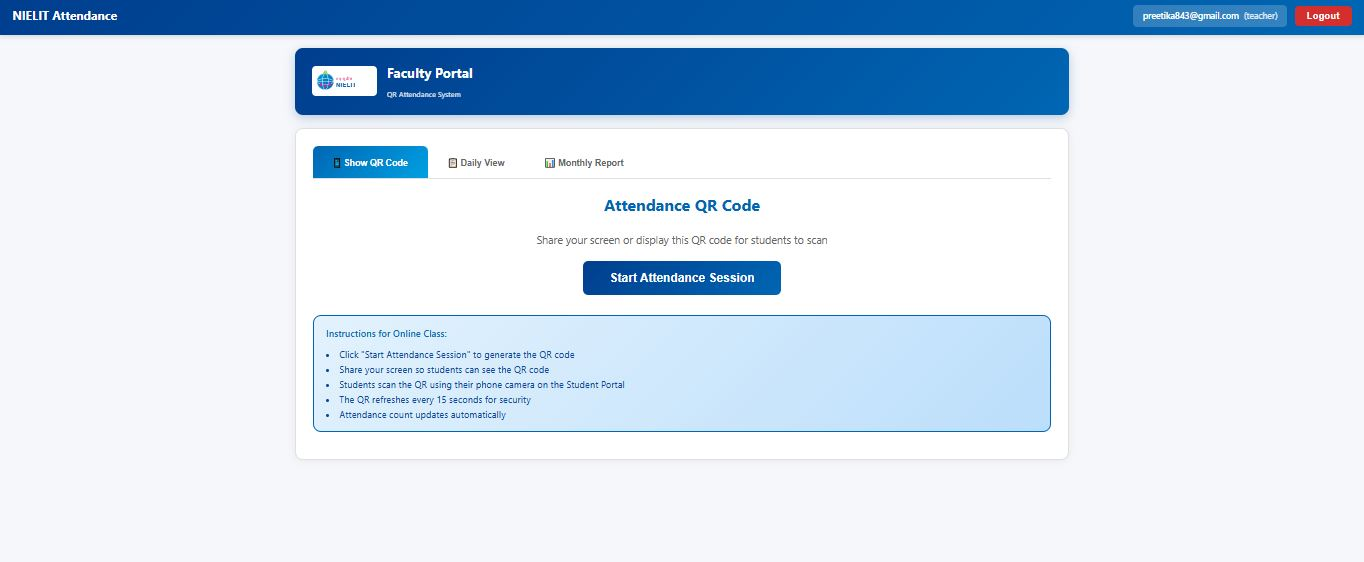
\includegraphics[width=0.65\linewidth]{Assets/second.JPG}
   \caption{Faculty Portal: Teacher dashboard showing QR Code generation, daily view, and monthly report tabs.}
   \label{fig:faculty_portal}
\end{figure}

\begin{figure}[H]
   \centering
   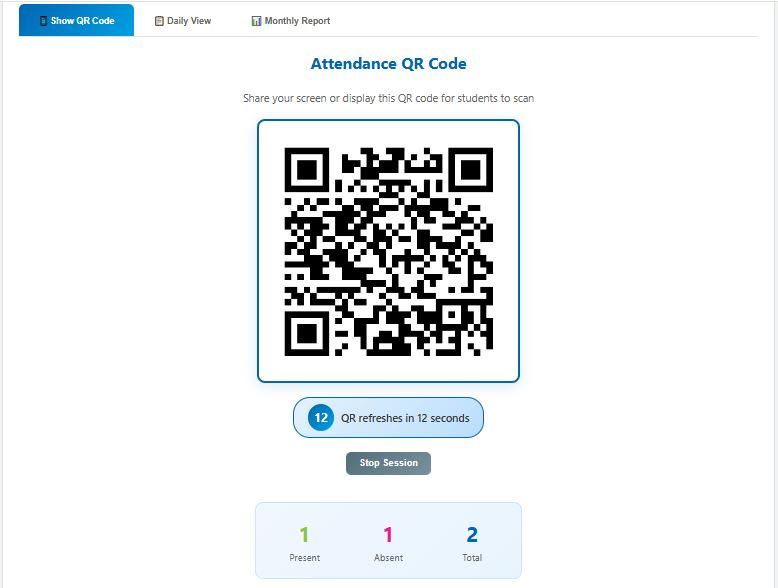
\includegraphics[width=0.65\linewidth]{Assets/third.JPG}
   \caption{QR Attendance Session: Active QR code display with real-time Present/Absent/Total counters.}
   \label{fig:qr_session}
\end{figure}

\begin{figure}[H]
   \centering
   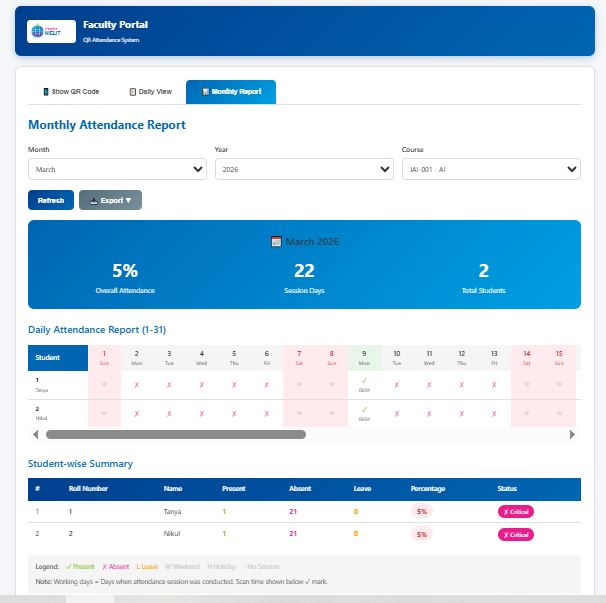
\includegraphics[width=0.65\linewidth]{Assets/fourth.JPG}
   \caption{Monthly Attendance Report: Calendar-style grid showing daily attendance status for all students.}
   \label{fig:monthly_report}
\end{figure}

\begin{figure}[H]
   \centering
   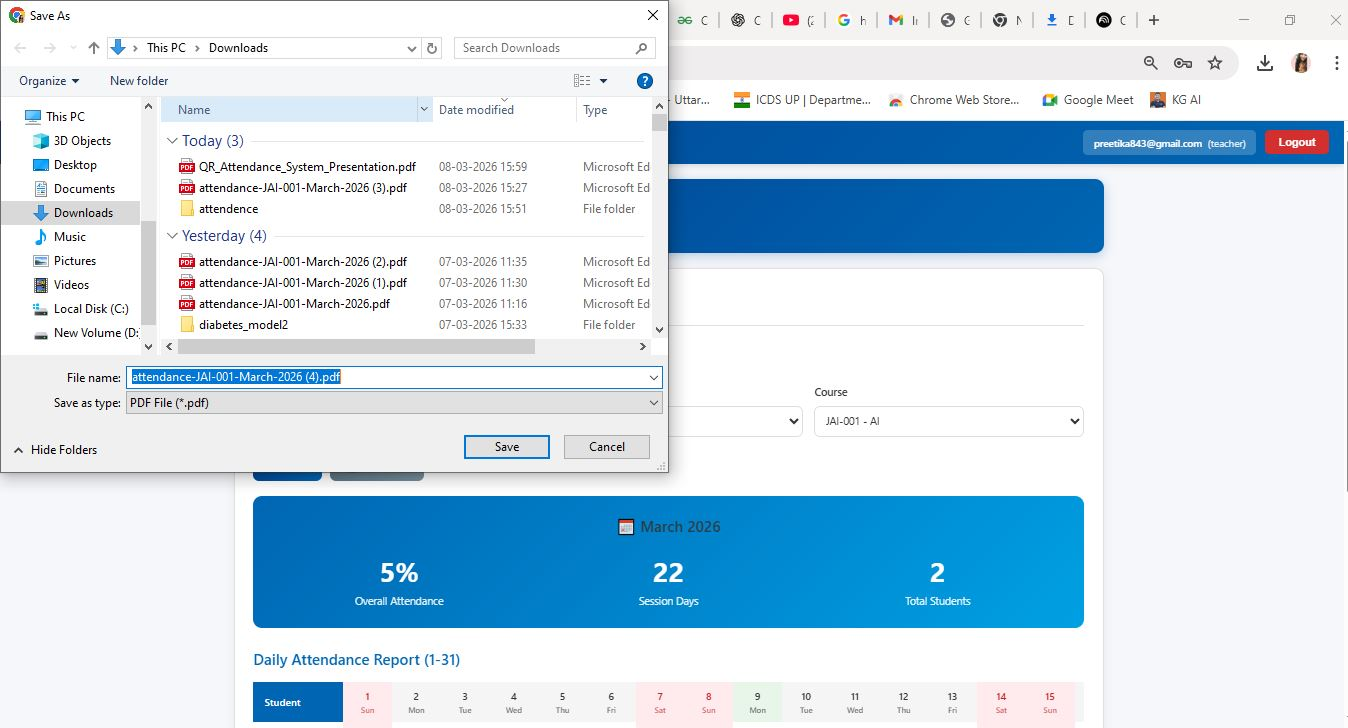
\includegraphics[width=0.65\linewidth]{Assets/fifth.JPG}
   \caption{PDF Export: Generated monthly attendance PDF with NIELIT branding and calendar-style layout.}
   \label{fig:pdf_export}
\end{figure}

\begin{figure}[H]
   \centering
   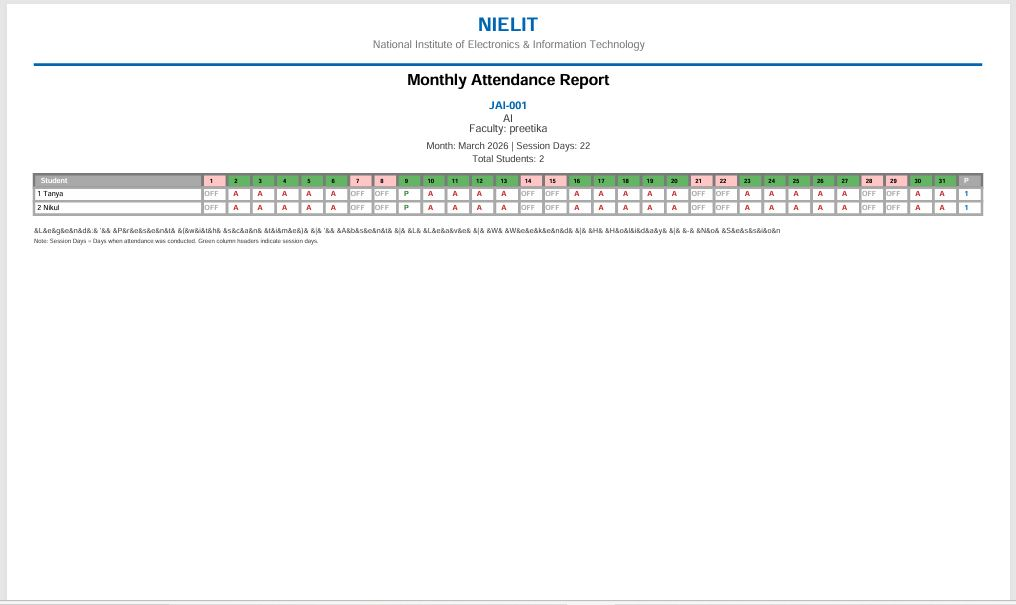
\includegraphics[width=0.65\linewidth]{Assets/sixth.JPG}
   \caption{Student Portal: QR scanning interface for marking attendance using mobile camera.}
   \label{fig:student_portal}
\end{figure}

\begin{figure}[H]
   \centering
   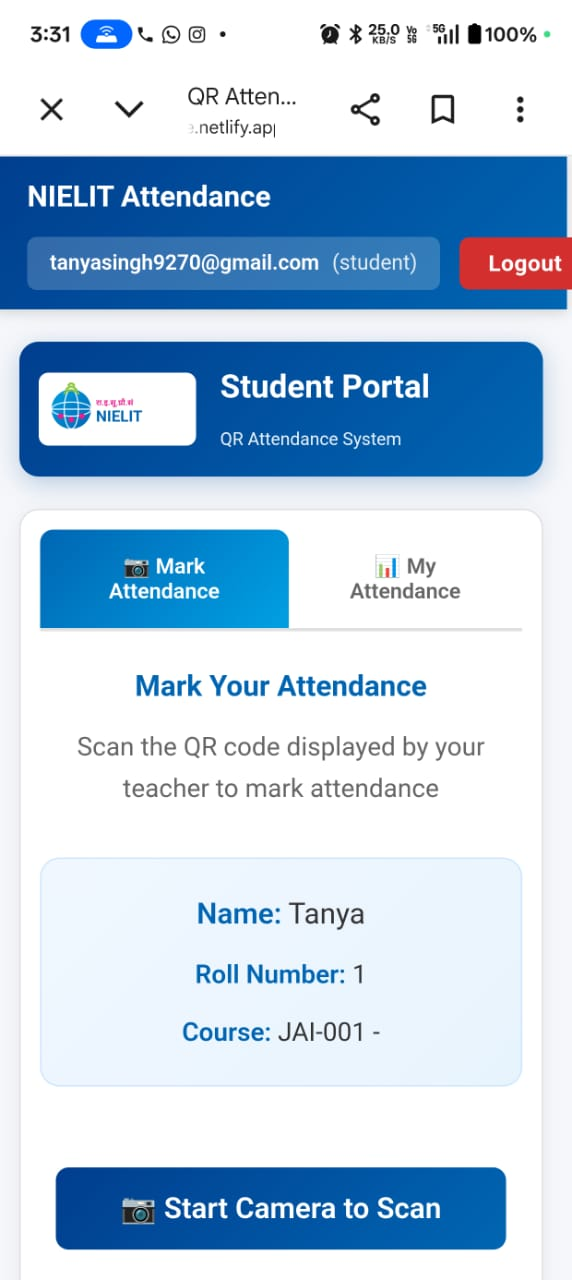
\includegraphics[width=0.65\linewidth]{Assets/whatsapp1.jpeg}
   \caption{Mobile QR Scanning: Student scanning QR code from mobile device to mark attendance.}
   \label{fig:mobile_scan}
\end{figure}

\begin{figure}[H]
   \centering
   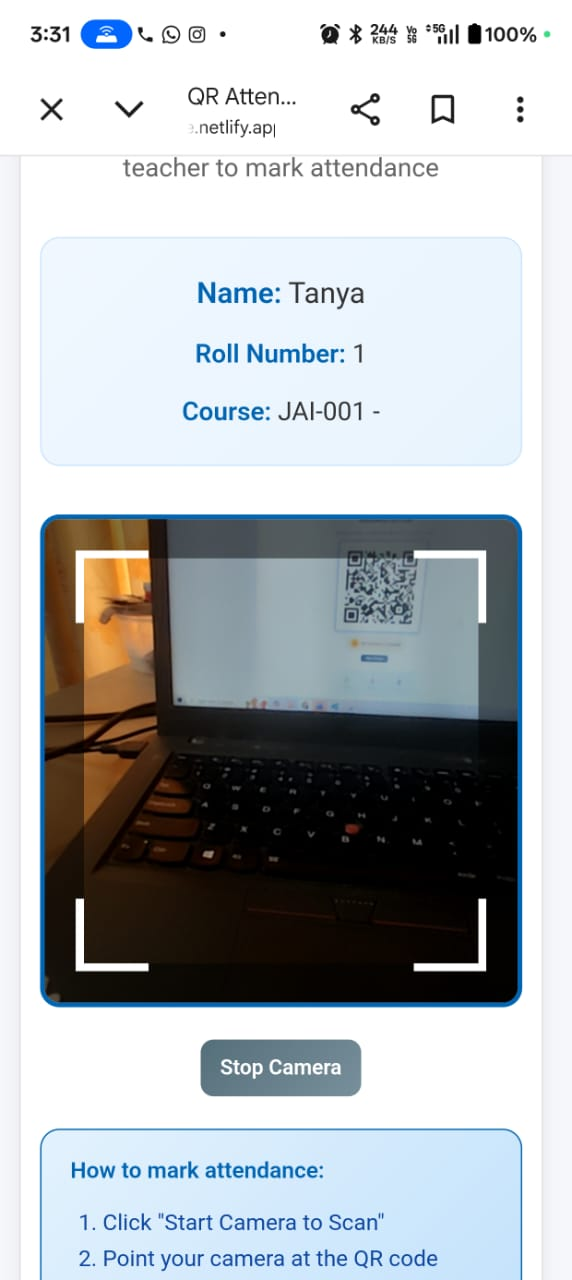
\includegraphics[width=0.65\linewidth]{Assets/whatsapp2.jpeg}
   \caption{Attendance Confirmation: Successful attendance marking confirmation on student's device.}
   \label{fig:attendance_confirm}
\end{figure}

\begin{figure}[H]
   \centering
   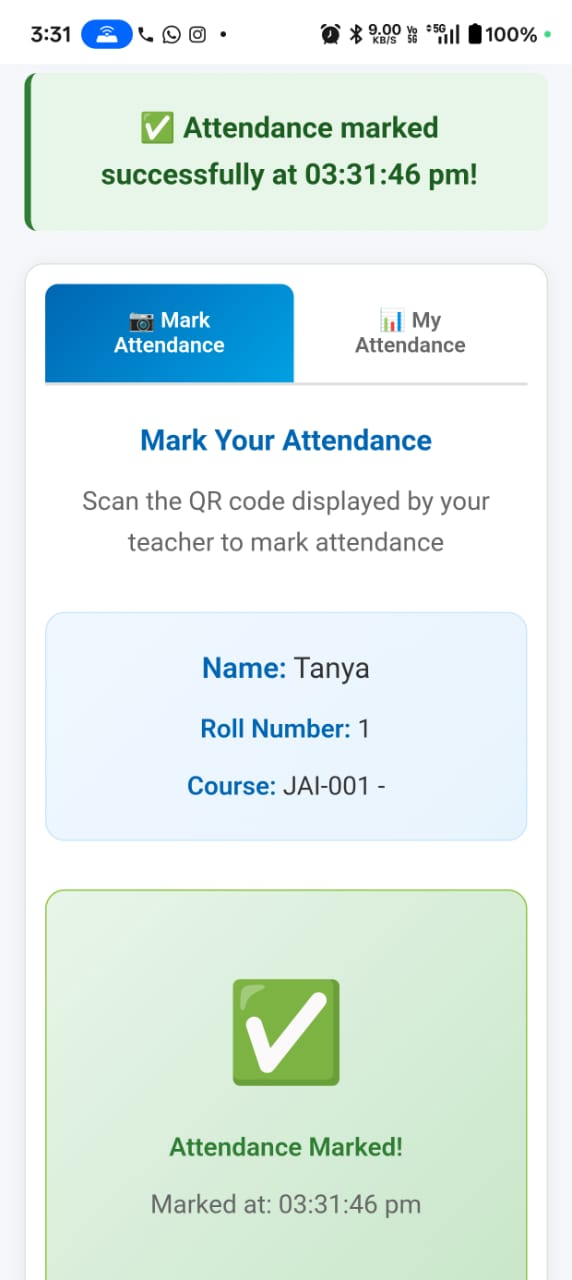
\includegraphics[width=0.65\linewidth]{Assets/whatsapp3.jpeg}
   \caption{Additional system view showing the application in use.}
   \label{fig:additional_view}
\end{figure}


% ---------------------------------
\chapter{OUTCOMES AND KEY LEARNINGS}
\label{ch:outcomes}
% ---------------------------------

\section{Project Outcomes}
\label{sec:outcomes}

\begin{enumerate}
    \item Successfully developed and deployed a fully functional QR-based attendance management system.
    \item Eliminated the possibility of proxy attendance through 15-second rotating QR codes with 30-second validation window.
    \item Achieved real-time attendance tracking with exact scan timestamps for complete audit trail.
    \item Built a multi-role system serving Admins, Teachers, and Students with appropriate access controls.
    \item Implemented automated monthly report generation in both PDF (calendar-style) and CSV formats.
    \item Deployed the application on cloud infrastructure ensuring 24/7 accessibility from any device.
    \item Created a responsive web application that works seamlessly on both desktop and mobile devices.
    \item Designed a scalable database schema with 8 migration files supporting multiple courses and teachers.
\end{enumerate}

\section{Key Learnings}
\label{sec:learnings}

\begin{itemize}
    \item \textbf{Supabase as a Backend Platform:} Gained hands-on experience with Supabase's comprehensive platform including Auth, PostgreSQL, Edge Functions, and Row Level Security. Learned how to leverage a Backend-as-a-Service for rapid application development.

    \item \textbf{Serverless Architecture:} Understood the benefits and constraints of serverless computing through Supabase Edge Functions running on Deno. Learned about cold starts, execution limits, and stateless function design.

    \item \textbf{React SPA Development:} Deepened knowledge of React component architecture, hooks (useState, useEffect, useRef), and client-side routing with React Router v6.

    \item \textbf{QR Code Technology:} Learned about QR code encoding, generation (using the `qrcode'' library), and camera-based scanning (using `html5-qrcode''). Understood how time-validation prevents replay attacks.

    \item \textbf{JWT Authentication:} Gained practical experience implementing token-based authentication, understanding token structure, expiry handling, and role-based authorisation patterns.

    \item \textbf{PDF Generation:} Learned client-side PDF generation using jsPDF, including manual layout calculations for landscape orientation, color management, font handling, and creating complex calendar-style grids.

    \item \textbf{CI/CD and Deployment:} Gained experience with Netlify's automatic deployment pipeline triggered by Git pushes, environment variable management, and production build optimisation with Vite.

    \item \textbf{Database Design and Migrations:} Practised incremental schema evolution through migration files, learned about constraint management, composite keys, and UUID-based user identification.
\end{itemize}

\section{Challenges Faced}
\label{sec:challenges}

\begin{itemize}
    \item \textbf{QR Timing Synchronisation:} Ensuring accurate time comparison between the teacher's QR generation timestamp and the student's scan time required careful handling of clock differences.

    \item \textbf{UUID-Integer Mapping:} Supabase Auth uses UUIDs for user IDs, while the students table originally used integer IDs. This required implementing a lookup mechanism via auth metadata.

    \item \textbf{Timezone Handling:} Scan timestamps stored in UTC needed proper conversion to IST (Indian Standard Time) for display. JavaScript Date handling across timezones was a recurring challenge.

    \item \textbf{PDF Layout Complexity:} Creating a calendar-style monthly grid in jsPDF required manual pixel-level layout calculations for 31+ columns, row heights, colour fills, and text positioning.

    \item \textbf{Mobile Camera Access:} Modern browsers require HTTPS for camera access on mobile devices. During development, this required configuring proper host settings.

    \item \textbf{Data Format Mismatches:} The backend API response format didn't directly match what the frontend components expected, requiring data transformation layers in the API client.

    \item \textbf{Database Schema Evolution:} As requirements evolved, the database schema needed multiple migrations to support features like per-course roll number uniqueness and multiple course enrollment.
\end{itemize}

\section{Testing Results}
\label{sec:testing}

\begin{table}[H]
\centering
\caption{Test Cases and Results}
\label{tab:test_cases}
\begin{tabular}{|p{4.5cm}|p{5cm}|c|}
    \hline
    \textbf{Test Case} & \textbf{Expected Result} & \textbf{Status} \\
    \hline
    Student scans valid QR within 15s & Attendance marked, timestamp recorded & Pass \\
    \hline
    Student scans expired QR (>30s) & Error: QR expired & Pass \\
    \hline
    Same student scans twice same day & Returns `already\_marked'' & Pass \\
    \hline
    Student scans wrong course teacher QR & Error: course\_mismatch & Pass \\
    \hline
    Teacher views monthly report & Calendar grid with P/A/Weekend markers & Pass \\
    \hline
    Export monthly PDF & Landscape PDF with NIELIT branding & Pass \\
    \hline
    Admin creates teacher + course & Auth user + course record created & Pass \\
    \hline
    Admin deletes student & Student + auth user + profile removed & Pass \\
    \hline
    Mobile phone camera QR scanning & Camera opens, decodes QR successfully & Pass \\
    \hline
\end{tabular}
\end{table}


% ---------------------------------
\chapter{CONCLUSION AND FUTURE SCOPE}
\label{ch:conclusion}
% ---------------------------------

\section{Conclusion}
\label{sec:conclusion}

The QR Attendance System developed during this NIELIT internship successfully demonstrates a modern, secure, and efficient approach to student attendance management. By leveraging dynamic QR codes with strict time validation, the system effectively eliminates the possibility of proxy attendance --- a persistent problem with traditional methods.

The application provides a complete solution covering the entire attendance lifecycle: from user management and session creation to real-time marking, daily/monthly reporting, and PDF export. The three-portal architecture ensures that each user role --- Administrator, Teacher, and Student --- has a tailored interface optimised for their specific needs.

The project has been fully deployed on cloud infrastructure (Netlify + Supabase), making it accessible from any device with internet connectivity. The serverless architecture ensures low operational costs while maintaining reliability and scalability.

This internship provided invaluable hands-on experience in full-stack web development, modern cloud services, database design, and production deployment --- skills that are directly applicable to industry software development.

\section{Future Scope}
\label{sec:future_scope}

Several enhancements can be made to the system in the future:

\begin{enumerate}
    \item \textbf{Biometric Integration:} Adding fingerprint or face recognition as an additional verification layer.
    \item \textbf{Geofencing:} Using GPS coordinates to ensure students are physically within the classroom.
    \item \textbf{Analytics Dashboard:} Charts and graphs showing attendance trends, peak times, and patterns.
    \item \textbf{Push Notifications:} Alerting students about attendance sessions and low attendance warnings.
    \item \textbf{Multi-Institution Support:} Extending the system to support multiple NIELIT centres.
    \item \textbf{Offline Mode:} Allowing attendance marking when internet connectivity is temporarily unavailable.
    \item \textbf{Integration APIs:} Connecting with institutional ERP systems for unified student management.
    \item \textbf{Automated Reports:} Scheduled email delivery of monthly attendance reports to administrators.
\end{enumerate}

\end{document}
